\documentclass[12pt]{article}\usepackage[margin=1in]{geometry}\usepackage{amsmath,amssymb,amsthm,graphicx,natbib,microtype}\newtheorem{theorem}{Theorem}\newtheorem{corollary}[theorem]{Corollary}
\title{Outward Loewner Transport Guards\\\large Rigorous Cross-Assembly Congruence from Spectral-Norm Radii}\author{Prime Dynamics Theory Program}\date{July 2026}
\begin{document}\maketitle
\begin{abstract}
The RH-115 audit showed that independently rounded Gram assemblies cannot be
fused without an outward transport loss.  We give the exact loss.  Suppose
$\|G-\widehat G\|\leq r_G$ and analogously for $D,G',D'$.  A numerical Gram
slack for $\widehat G'-aS^*\widehat GS$ becomes rigorous after subtracting
$r_{G'}+a\|S\|^2r_G$.  A numerical tail slack for
$bS^*\widehat DS+\delta S^*\widehat GS-\widehat D'$ becomes rigorous after
subtracting $r_{D'}+\|S\|^2(br_D+\delta r_G)$.  Both guards are sharp for
scalars.  A 4,096-instance enclosure audit has zero false certifications.
The theorem closes the validation logic but does not supply physical
all-level radii.
\end{abstract}
\section{Outward comparison theorem}
\begin{theorem}[Outward gauged Loewner guards]\label{thm:guards}
Assume spectral-norm enclosures for $G,D,G',D'$ with radii
$r_G,r_D,r_{G'},r_{D'}$.  Let
\[
\widehat\mu_G=\lambda_{\min}(\widehat G'-aS^*\widehat GS),
\]
\[
\widehat\mu_D=\lambda_{\min}(bS^*\widehat DS+delta S^*\widehat GS-\widehat D').
\]
If
\[
\widehat\mu_G\geq r_{G'}+a\|S\|^2r_G,
\]
then $G'\succeq aS^*GS$.  If
\[
\widehat\mu_D\geq r_{D'}+\|S\|^2(br_D+\delta r_G),
\]
then $D'\preceq bS^*DS+\delta S^*GS$.
\end{theorem}
\begin{proof}
Write each exact matrix as its approximation plus an error.  The minimum
eigenvalue changes by at most the spectral norm of the total error.  Under
congruence, $\|S^*ES\|\leq\|S\|^2\|E\|$.  Applying the triangle inequality
gives the two guards \citep{Moore1966,HornJohnson1991}.
\end{proof}

\section{Sharpness}
In dimension one, choose every enclosure error with the sign that reduces
the exact slack.  Then the exact Gram slack equals
$\widehat\mu_G-r_{G'}-a|S|^2r_G$, and the exact tail slack equals
$\widehat\mu_D-r_{D'}-|S|^2(br_D+\delta r_G)$.  Hence no smaller universal
guard follows from norm radii alone.

\section{Audit and route consequence}
We sample 4,096 positive source pairs, gauges, factors, radii over five
decades, and independent symmetric perturbations at their enclosure
boundaries.  Every generated instance has numerical reserve beyond the
required guard.  All 4,096 are certified and direct access to the hidden
exact matrices finds zero false certifications.  A scalar adversarial record
attains both guard boundaries to error below $10^{-12}$.
\begin{figure}[h]\centering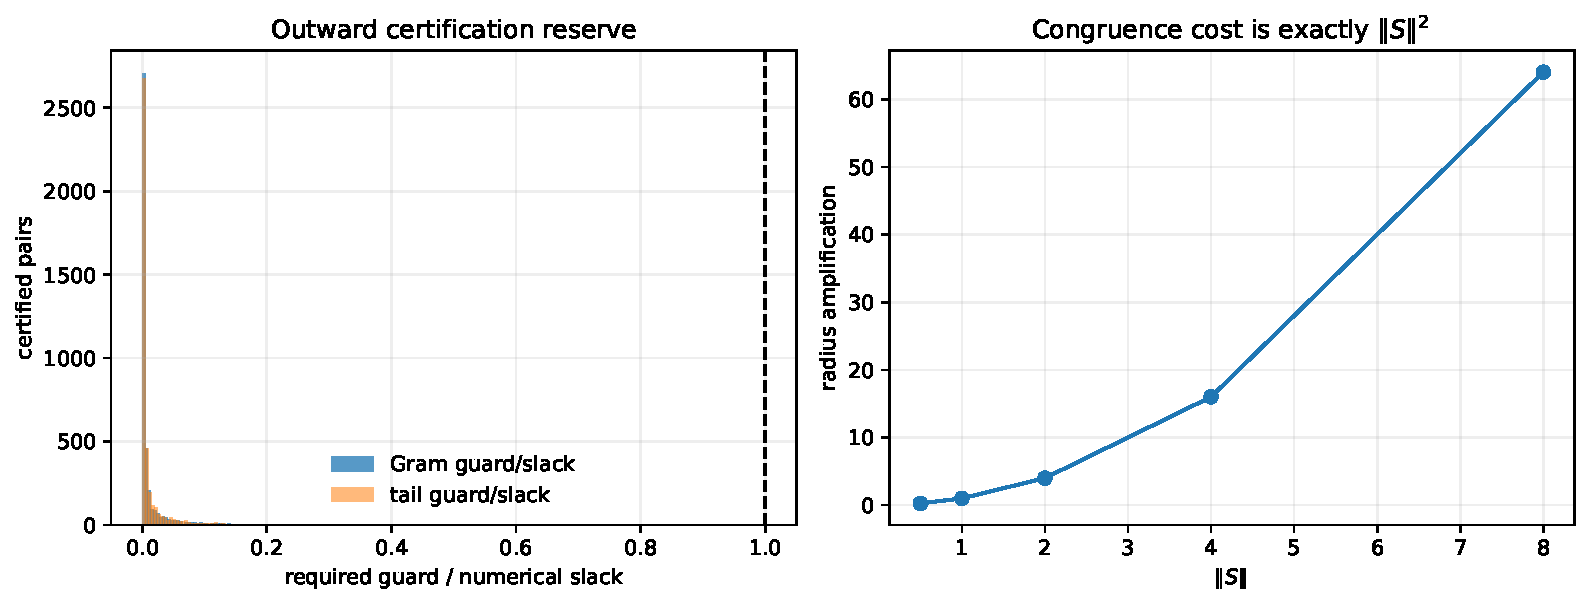
\includegraphics[width=\textwidth]{figures/outward_loewner_transport_guards.pdf}\caption{Certification reserve and the exact squared-gauge amplification of source radii.}\end{figure}

RH-127 resolves the formal cross-assembly issue exposed in RH-115: a future
validated recurrence may combine independent paths if it archives these
radii and guards.  It does not retroactively certify old unguarded paths and
does not prove uniform physical radii.  No Stage A, Hilbert--Polya,
zeta-zero, or Riemann Hypothesis conclusion is claimed.
\bibliographystyle{plainnat}\bibliography{references}\end{document}
